\documentclass{beamer}

\mode<presentation>
{
  \usetheme{CambridgeUS}      % or try Darmstadt, Madrid, Warsaw, ...
  \usecolortheme{default} % or try albatross, beaver, crane, ...
  \usefonttheme{default}  % or try serif, structurebold, ...
  \setbeamertemplate{navigation symbols}{}
  \setbeamertemplate{caption}[numbered]
  \setbeamertemplate{bibliography item}[text]
} 

\usepackage[english]{babel}
\usepackage[utf8x]{inputenc}
\usepackage[document]{ragged2e}
\usepackage{amsmath}

\usepackage{listings}
\usepackage{color}

\lstset{frame=tb,
  language=C,
  breaklines=true,
}

\title[Applied Parallel Programming]{Bilinear Interpolation Upsampling on CUDA}
\subtitle{Project Phase-I}
\author{Bilgin AKSOY}

\institute{\bf Informatics Enstitute}
\logo{
\includegraphics[scale=0.2]{./Figures/iilogo.png}}
\date{$12^{\text{th}}$ Nov 2017}

\begin{document}

	\begin{frame}
	  \titlepage
	\end{frame}

% Problem definitons
\section{Introduction}

	\begin{frame}{Problem}
		
		\begin{itemize}
		  \item A deep network for object segmentation.  
		  \item \justifying This network has 5 two-by-two max-pooling layer, each of which downsamples its input by factor two. 
		\end{itemize}
		\begin{figure}
		  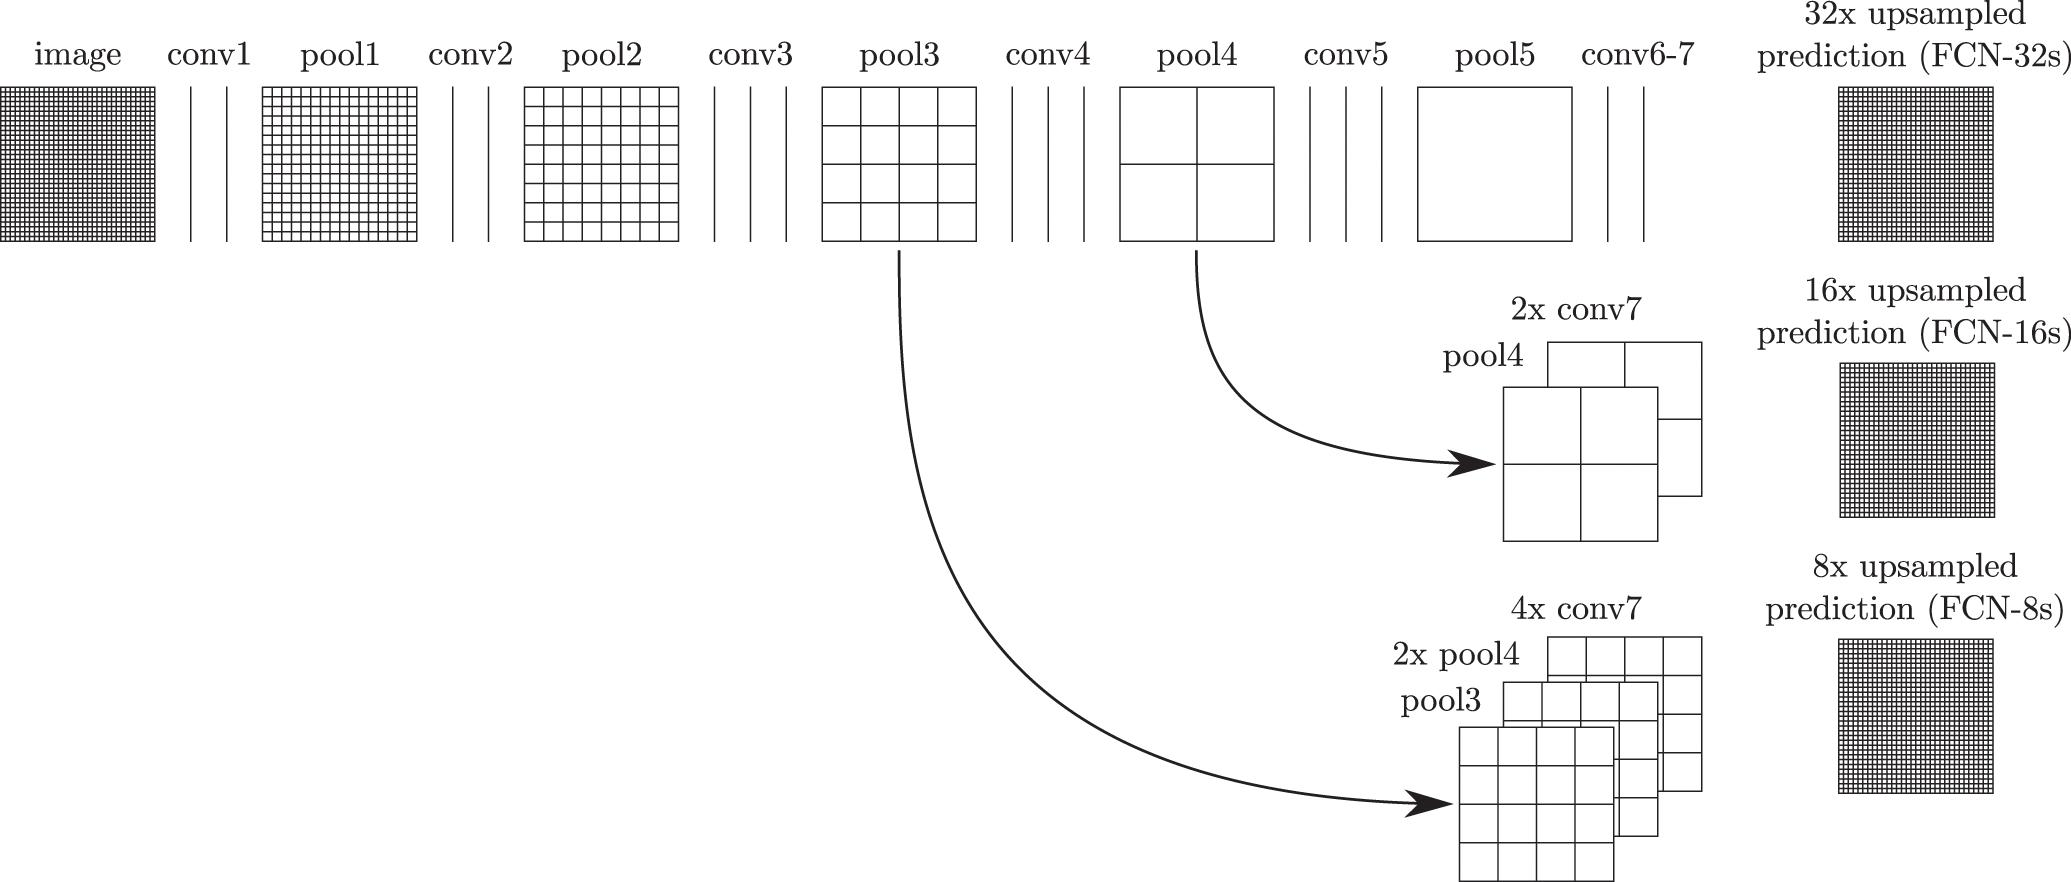
\includegraphics[scale=0.15]{./Figures/DAGnet.jpg}
		  \caption{\label{fig:DAGnet}Network Architecture-Long et al.\cite{long2015fully}}
		\end{figure}	
	\end{frame}
	%next slide
	\begin{frame}{Problem (cont'd)}
		\begin{itemize}
				\item After pool3, the activation size have been reduced by factor $8= 2^3 $.
				\item After pool4, the activation size have been reduced by factor $16= 2^4 $.
				\item After pool5, the activation size have been reduced by factor $32= 2^5 $.
		\end{itemize}
		\vskip 5 cm
	\end{frame}
	%next slide
	\begin{frame}{Problem (cont'd)}
		\begin{itemize}
			\item \justifying Sum three activations and calculate the error(loss) and back-propagate the error at the end of the final layer.
		\end{itemize}
		\begin{figure}
			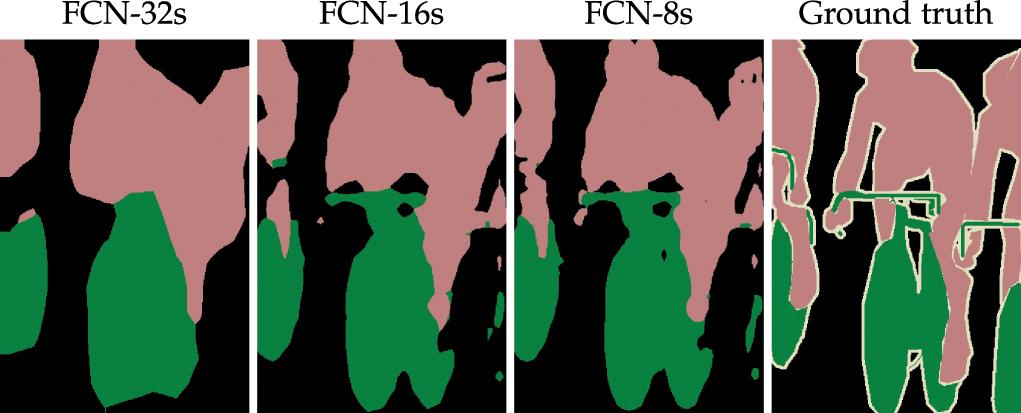
\includegraphics[scale=0.15]{./Figures/fcn_output.jpg}
			\caption{\label{fig:fcn_output}Activations of Pooling Layers-Long et al.\cite{long2015fully}}
		\end{figure}
	\end{frame}
	%next slide
	\begin{frame}{Problem (cont'd)}
		\begin{itemize}
			\item I will implement a bilinear interpolation upsampling kernel and my kernel will not only upsample the activations but also produce the final result by summing the activations.
		\end{itemize}
	\end{frame}
	
%Literature Survey	
\section{Literature}
	%next slide
	\begin{frame}{Literature Survey}
		\begin{itemize}
			\item \justifying \textbf{\underline{Bilinear Interpolation:}} Bilinear interpolation is used to know values at 	random position from the weighted average of the 	four closest pixels to the specified input coordinates, and assigns that value to the output coordinates.\cite{fadnavis2014image}  \eqref{equ:bilinear}
		\end{itemize}
	\end{frame}
	%next slide
	\begin{frame}
		\begin{figure}
			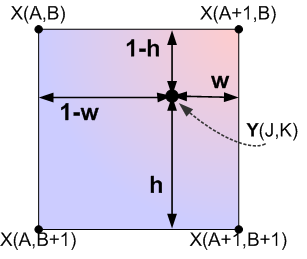
\includegraphics[scale=0.5]{./Figures/bilinear_interpolation.png}
			\caption{\label{fig:bilinear_img}Image from \url{https://www.giassa.net/?page_id=240}\cite{bilinear_img}}
		\end{figure}
		\begin{multline}\label{equ:bilinear}
			Y(J,K)=(1-W)(1-H)X(A,B)+(W)(1-H)X(A+1,B)+\\(1-W)(H)X(A,B+1)+(W)(H)X(A+1,B+1)
		\end{multline}\vskip 4 cm
	\end{frame}
	%Next slide
	\begin{frame}[fragile]
	\begin{block}{OpenCV CPU}		
	\end{block}
		\begin{lstlisting}
		void 	cv::resize (
		InputArray src, OutputArray dst, Size dsize, double fx=0, double fy=0, int interpolation=INTER_LINEAR
		)
		\end{lstlisting}
	
		\begin{block}{OpenCV GPU}		
		\end{block}
			\begin{lstlisting}
			
			void cv::cuda::resize	(
			InputArray 	src, OutputArray 	dst, Size 	dsize, double 	fx = 0, double 	fy = 0, int 	interpolation = INTER_LINEAR, Stream & 	stream =Stream::Null() 
			)	
			\end{lstlisting}
		\end{frame}

%References
\section{References}
	%next slide
	\begin{block}{References}
	\end{block}
	\bibliography{./References/ref.bib}
	\bibliographystyle{ieeetr}

\end{document}